\question What is wrong with the following \"proof\"? \newline

\textbf{False Claim}: If every vertex in an undirected graph has degree 
at least 1, then the graph is connected.\newline

\begin{proof} We use induction on the number of vertices $n \geq 1$.\newline

\textit{Base case}: There is only one graph with a single vertex and it 
has degree 0. Therefore, the base case is vacuously true, since the 
if-part is false.\newline

\textit{Inductive Hypothesis}: Assume the claim is true for some $n 
\geq 1$.\newline

\textit{Inductive Step}: We prove the claim is also true for $n + 1$. 
Consider an undirected graph on $n$ vertices in which every vertex has 
degree at least 1. By the inductive hypothesis, this graph is connected. 
Now add one more vertex $x$ to obtain a graph on $(n + 1)$ vertices, 
as shown below.

\begin{figure}[h]
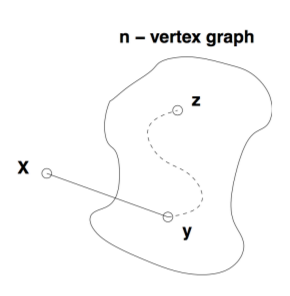
\includegraphics{build_up_error}
\centering
\end{figure}
 
All that remains is to check that there is a path from $x$ to every 
other vertex $z$. Since $x$ has degree at least 1, there is an edge 
from $x$ to some other vertex; call it $y$. Thus, we can obtain a 
path from $x$ to $z$ by adjoining the edge ${x, y}$ to the path from 
$y$ to $z$. This proves the claim for $n + 1$.
\end{proof}

\begin{solution}
Build up error! Always start with the $n+1$ case, \textbf{especially} 
when working with graphs. If we start with a graph that has $n+1$ 
vertices, is it possible to work with such a graph that removing one 
vertex will create a graph with $n$ vertices, but which is disconnected?
\end{solution}

\clearpage